%-----------------------
%\documentclass[a4paper,twoside=false,abstract=false,numbers=noenddot,
%titlepage=false,headings=small,parskip=half,version=last]{scrartcl}
\documentclass[11pt, titlepage, a4paper]{article}
%-----------------------
\usepackage[T1]{fontenc}
\usepackage[english]{babel}
\usepackage[utf8]{inputenc}
\usepackage{csquotes}
\usepackage{amssymb, graphicx, fancyhdr}
\usepackage{abstract}
\usepackage{a4wide}
%\usepackage[utf8]{inputenc}
\usepackage[T1,T2A]{fontenc}
%\usepackage[english]{babel}
\usepackage{stringenc}
\usepackage{pdfescape}
%\usepackage[subfig]
\usepackage{float}
%\usepackage{listing}
\usepackage{longtable}
\usepackage{multirow}
\usepackage{textcomp}
\usepackage{lmodern}
\usepackage{amsmath}
\usepackage{amssymb}
\usepackage{wrapfig}
\usepackage{algpseudocode}
\usepackage[hidelinks]{hyperref}
\usepackage{mathtools}
\usepackage{tikz}
\graphicspath{{./}}
\usepackage{paralist}
\usepackage{mdframed} % figure box frame
\usepackage{graphicx}


\usetikzlibrary{matrix,arrows,decorations.pathmorphing}
%-----------------------
%\usepackage{./lib/header}
%\usepackage{./lib/probability}
%-----------------------
\title{Detecting Anomaly in the NSL-KDD Dataset \\ from Spectral Analysis}

\author{Kim Seonghyun \\{\small}

\date{\today}

\begin{document}
\maketitle
%\makeatletter
%\title{Detecting Anomaly in NSL KDD 99 Dataset from Spectral Analysis} \let\Title\@title
%\author{Kim Seonghyun} \let\Author\@author
%\makeatother
%Low-Power In situ Activity Classification using Wireless Sensor Network Eartag Devices on Livestock
% honours students will want to override the \degreetext variable with
% something appropriate like that here:
%\renewcommand{\degreetext}{}
\titlepage
%\input{frontstuff/letter}
%\input{frontstuff/acknowledge}
\section{Abstract}
Network intrusion detection system provides crucial factors for network security analysis.
The report deals with the problem of detect intrusion connections by analysing known intrusions and unknown anomalous connections.
It proposes clustering approach for detecting point and collective anomalies by analyzing similarity of the multi-dimensional data, with spectral clustering and expection maximization algorithm.
The experiments on NSL-KDD 99 dataset validate the effectiveness in detecting both known intrusionsand unknown anomalies.

%\tableofcontents
% comment out these as required for your discipline
%\listoffigures
%\listoftables

%-----------------------
\chapter{Introduction}

Anomaly detection refers to the problem of finding patterns in data that do not conform to expected behavio. For example, an anomalous traffic pattern in a computer network could mean that a hacked computer is sending out sensitive data to an unauthorized destination. In this individual course, the aims of the study is to research and to develop the algorithm to detect novel network attack type.

\begin{itemize}
\item Chapter 2
\item Chapter 3
\item Chapter 4
\end{itemize}

\section{Related works}
% What is different approaches/alternative to NIDS has there been before?
Semi-supervised or unsupervised approaches are preferred in Anomaly Detection\cite{chandola09} because labeled data corresponding to normal behaviour is available while labels for intrusions are not. 
Different approaches to network intrusion detection systems, such as \begin{inparaenum}[\itshape a\upshape)] \item statistical profiling using histogram, \item mixture of models, \item neural networks, \item support vector machines, and \item rule-based system\end{inparaenum}. NSL-KDD99 Dataset is mainly used in this subject\cite{tavallaee09}. 
The relevance of each feature in the data set is also studied\cite{olusola10} \cite{kayacik05}. 

% In what way they differ from each other
The rule-learning engine RIPPER and ToolDiag is applied to the training data with feature labeled as normal or intrusion and generate rules for classification. 
Minnesota Intrusion Detection System selected LOF detection method. 
Also fuzzy based methods are proposed.

%% In what way they differ from what we do here
%I assumes the data 
%to decide k value.
%I uses histogram and mixture models to measure its similarity.

% Why is our approach better than what has done before. does it solve a partly new aspect of the problem or does it simply perform better
In this report, I use spectral clustering algorithm for intrusion detection. 
The advantages of spectral clustering is it only requires pairwise similarity of data points. 

\begin{table}[h]
%\begin{tabular}{|r|l|}
%\end{tabular}
(table)
\caption{Intrusion detection approaches}
\label{fig:refSingleRobot1}
\end{table}


\newpage
\section{Connection Similarity}
\label{sec:connectionsimilarity}
The problem of comparing network connection similarity has been an important problem. %\cite{}
Since there is not only one normal state, I generated mixture models for normal connections for each protocols and attributes.
After reviewing the families of proposed schemes, I indentified similarity and density approaches as the promising for the problem.
\newline
In Section~\ref{subsec:problemformulation}, I describe the problem.\newline
In Section~\ref{subsec:normalabnormalsimilarity}, I propose new approaches to measure similarity.\newline
In Section~\ref{subsec:densitysimilarity}, I describe density similarity measurement which is relied on the way of representatives of the clusters and threshold.\newline
%In Section~\ref{subsec:learningsimilarity}, I describe how the algorithm learn mixture models with training set.\newline

\subsection{Problem Formulation}
\label{subsec:problemformulation}
Given dataset, we can learn normal/abnormal mixture models, and estimate a density of normal connections from training set.
Anomalies can be detected by cluster algorithm based on affinity matrix which is computed by similarity score, or by comparing density of clusters against threshold.

\subsection{Normal and Abnormal Connection Similarity}
\label{subsec:normalabnormalsimilarity}
Two nodes are similar if their similarity to normal and abnormal mixture models are similar. 
Mixture models can be learned by EM algorithm. 
They compute the similarity score, log probability of each connections, under the model. 
The EM approach is guaranteed to converge to a local optimum on a given input. 
We define the similarity between two nodes using cosine distance of normal and abnormal similarity scores. 
I applied the EM algorithm seperately for 23 known classes, three protocols and 39 attributes. 
Each feature have different correlation to the result, so I give different weights on them \cite{olusola10}\cite{kayacik05}.
%Learned $234(=2 \times 3 \times 39)$ Gaussian mixture models in total.
%\begin{itemize}
%\item 2 : one for normal, one for abnormal.
%\item 3 : each per each protocol e.g.) udp, icmp, tcp.
%\item 39 : for all attributes.
%Since the data fit the gaussian and a sufficient number of data points are available to learn the parameters of the model, the model can be learned.

\begin{equation}
    sim(V, V') = \frac{A \cdot B}{|A| |B|}
\end{equation}

\subsection{Connection Density Similarity}
\label{subsec:densitysimilarity}
A cluster is abnormal if its density differs from density of known normal connections even though the cluster is similar to normal behaviour. 
For anomaly detection, only density of each cluster is compared with the density of known normal connections. 
If the density of a cluster is higher than a supposed density in the region, the cluster is classified as an anomaly. 
So it allows detecting unknown anomalies which is similar to known normal connections. 
In contrast to the known normal and abnormal connection similarity, it does not need to use known anomalies that appear in the training set. 
This is illustrated in (Figure) where one cluster over the distribution and threshold. 
We can also define threshold and adjust threshold if false-positive or false-negative is high. 

%\begin{equation}
%    d = \sum_X \sum_Y 
%\end{equation}
%\subsubsection{Measuring similarity}
%\label{subsec:densitysimilarity}
%Gaussian mixture models from training set helps to measure those two similarity per each connection.
%\begin{itemize}
%\item Similarity to known normal behavior.
%\item Similarity to known abnormal behavior.
%\end{itemize}


%\section{Experiments}
I performed experiments to evaluate the performances of similarity measures and algorithms in Section~\ref{sec:connectionsimilarity}.
\newline
In Section~\ref{subsec:datasetandsetup}, I describe the dataset that I used for the experiments.\newline
In Section~\ref{subsec:preprocessing}, I describe data pre-processing over the dataset.\newline
In Section~\ref{subsec:detectinganomalies}, I evaluate how successful the algorithms are in detecting different types of anomalies.

\subsection{Dataset and Setup}
\label{subsec:datasetandsetup}
The KDD 99 dataset is mainly used for a network-based intrusion detection algorithm evaluation \cite{tavallaee09}. 
I select the NSL-KDD dataset, which is an up-to-date version of the KDD 99 dataset, as an effective benchmark. 
% Since the NSL-KDD dataset solves issues in the KDD 99 dataset, I use the dataset as an effective benchmark. 
Its relevance of each feature in the dataset is also studied \cite{olusola10} \cite{kayacik05}. 
% All source code is on the Internet. 
% I use NSL-KDD99 Dataset for the report. 
% semi-supervised approach

\begin{figure}[htb2]
\begin{center}
%\begin{inparaenum}[\itshape a\upshape)]
%\item data preprocessing
%\item data transformation
%\item affinity matrix computation
%\item clustering
%\item outlier detection
%\end{inparaenum}
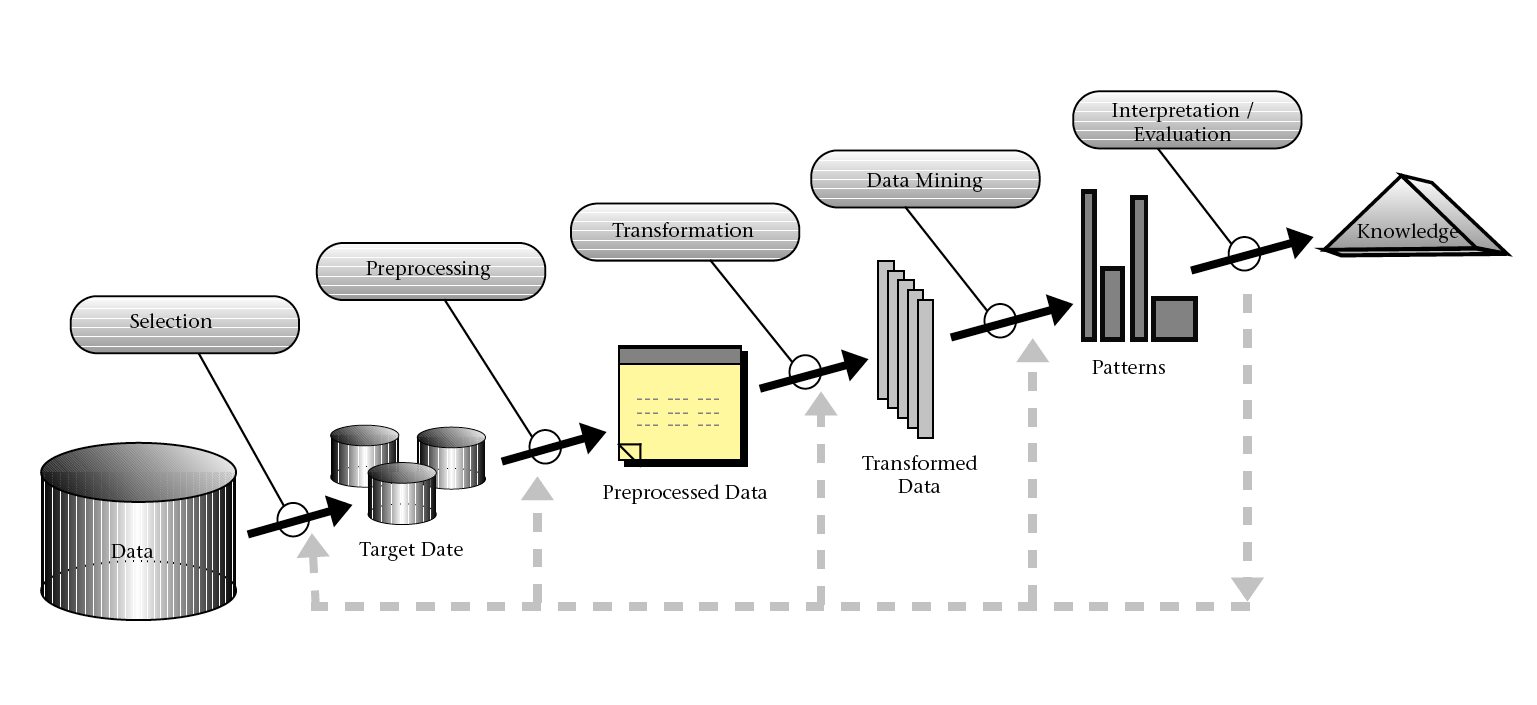
\includegraphics[width=5.5in,angle=0]{./sections/Fayyad96kdd-process.eps}
\end{center}
\caption{Overview of Knowledge Discovery System}
\label{fig:refSingleRobot1}
\end{figure}
The intrusion detection system should find specific kinds of abnormal traffic e.g. a denial of service (DoS) attack. 
It should check if these new sets of monitoring network traffic show similar properties as the original data or not as well. 
I construct the system similar to the knowledge discovery system \cite{fayyad96} because it is widely used among intrusion detection systems. 
A new approach to construct a pairwise similarity matrix is that it compares their probability in pairwise not its attributes directly. 
For this, the system includes gaussian mixture models for attributes and classes to calculate the probability for data point as I stated before. 
%The EM approach is used to fit those models and is guaranteed to converge to a local optimum on given input. 
With those components, we measure a score for each attributes, and those scores are weighted based on their importance in the dataset \cite{kayacik05}.
%to get 2D data where x-axis is a score for normal connection similarity and y-axis is a score for known abnormal connection similarity. 
The experiment suggests that such local optimum can effectively separate different connections and most of unknown classes. 
%\begin{figure}[htb2]
%\begin{center}
%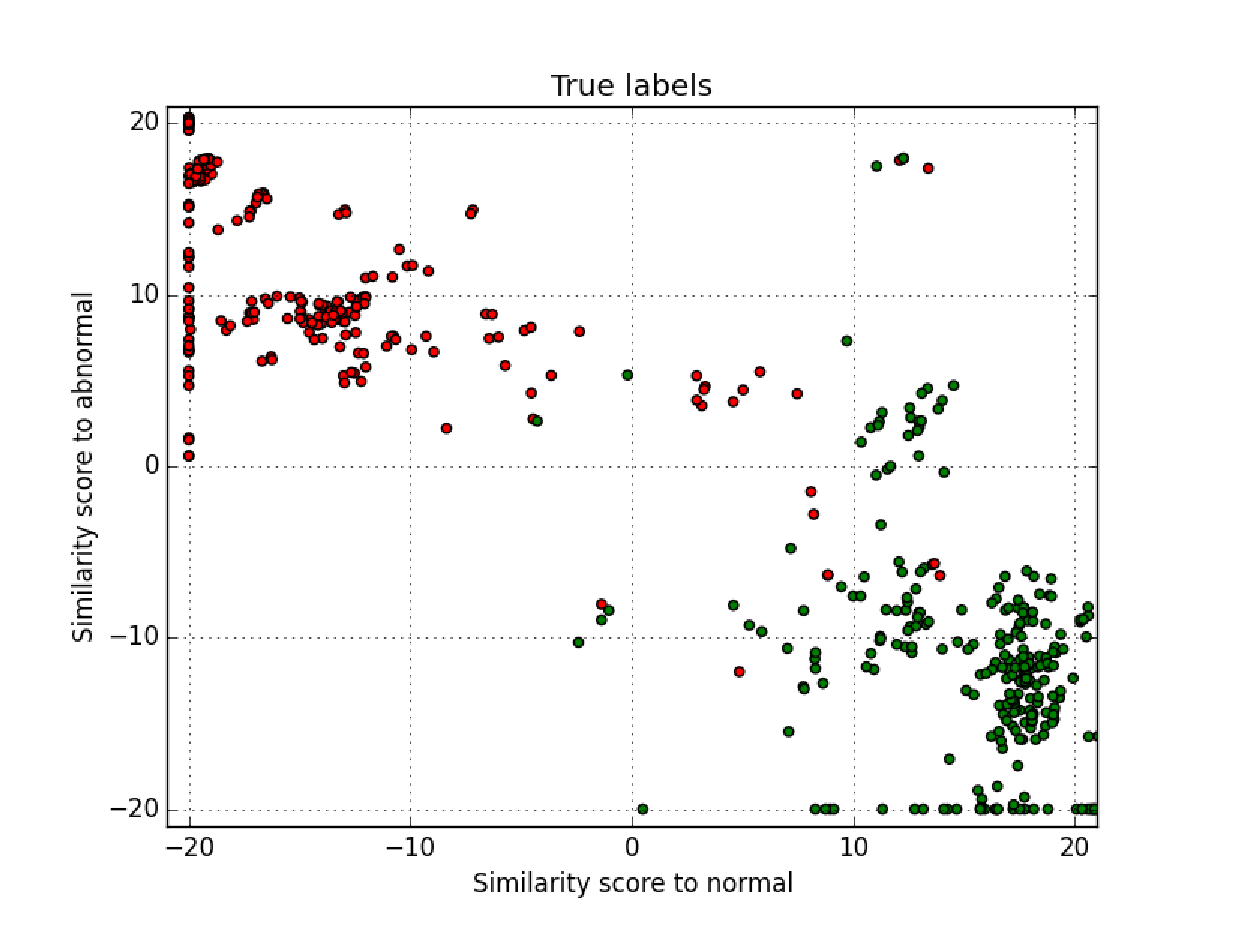
\includegraphics[width=3.5in,angle=0]{./sections/training20_only_true_.eps}
%\end{center}
%\caption{Similarity of normal and abnormal connections in training set.}
%% The left figure shows data points including known anomalies and the right known type of anomalies shows data points including unknown type of anomalies.} % I may show rest of data in appendix
%\label{fig:refSingleRobot1}
%\end{figure}

%In order for spectral anaysis, we need to make a sparse affinity matrix from transported data. 
%We can compute a sparse affinity matrix from a pairwise similarity matrix. 
After we have a pairwise similarity matrix, one way to convert similarity matrix to a sparse affinity matrix is that dealing with the affinities for $k$ nearest neighborhood, and set all other values for current data point to zero. 
I choose $k = 8$ because it is commonly used in spectral clustering approaches. 

% Altho require non-convex boundaries,
%\subsection{Computing affinity matrix}
%%The processing steps of the approach can be summerized as follows:
%%1) Training mixture model with training set containing records of both normal and anomalous connections.
%%2) The data are divided into different clusters for normal and anomalous connections using Spectral clustering algorithm.
%\subsubsection{Data pre-processing}
%\begin{itemize}
%\item categorical value to integer e.g.) service-type (ftp-data,http,etc).
%\item log of big number e.g.) duration, src-bytes.
%\end{itemize}
%\subsubsection{Affinity matrix computation}
%The data points are associated with each other by pairwise similarity.
%\begin{itemize}
%\item Construct similarity matrix with distance metric.
%\item Construct affinity matrix from similarity matrix with 8-nearest neighbors algorithm.
%\end{itemize}
%\subsection{Clustering}
%%\subsubsection{Number of clusters prediction}
%%Predict number of clusters based on the eigengap.
%%\subsubsection{Spectral clustering algorithm}
%%Normalized cut algorithm. \cite{jianbo00}
%%\subsubsection{Representative of clusters}
%%Clusters are represented by the mean and variance.
%\subsection{Detecting anomaly from clusters}
%%Distance based outlier detection is used.
%%\begin{itemize}
%%\item It do not require any prior knowledge.
%%\item k-nearest neighbor outlier detection algorithm. \cite{knorr00}
%%\end{itemize}

\subsection{Data Pre-processing}
\label{subsec:preprocessing}
A set of network connections $D_{\text{train}=(d_1, \cdots, d_{25192})}$ and $D_{\text{test}=(d_1, \cdots, d_{11850})}$ can be extracted from the NSL-KDD dataset. 
Each connection $D_i = (y, (\theta_{1}, \cdots, \theta_{39}))$ consists of a class label \\ 
$y \in Y=\{\text{normal},\text{anomaly}_1,\cdots,\text{anomaly}_{34}\}$ and a feature attributes $(\lambda_1,\cdots,\lambda_{39})$. 

$D_{\text{train}}$ has 22 types of known anomaly and $D_{\text{test}}$ has 39 types of known and unknown anomaly which can be seen in Table~\ref{fig:anomalyclasses}. 
Three of feature attributes are categorical values and ten of them are large numbers which requires data-preprocessing. 
Those of three are converted from categorical values into integer values. 
Preprocessing work applies log probability on large numbers $\hat{\lambda_{j}} = \log (\lambda_{j})$ where $j$ is an index of large number attributes. 
Each attributes' probability density can be learned by EM algorithm that can be used to calculate a log-likelihood score as it stated in Section~\ref{subsec:normalabnormalsimilarity}
\begin{table}[h]
\begin{center}
\begin{tabular}{| l | p{10cm} |}
\hline
Type of Attributes & Attributes Names \\
\hline
Categorical values (3) & attack, service, flag \\
\hline
Large numbers (10) & duration, src-bytes, dst-bytes, num-root, num-compromised, num-file-creations, count, srv-count, dst-host-count, dst-host-srv-count \\
\hline
Others (26) & land, wrong-fragment, urgent, hot, num-failed-logins, logged-in,su-compromised, root-sheel, su-attempted, num-shells, num-access-files, num-outbound-cmds, is-host-login, is-guest-login, serror-rate, srv-serror-rate, rerror-rate, same-srv-rate, diff-srv-rate, srv-diff-host-rate, dst-host-same-srv-rate, dst-host-diff-srv-rate, dst-host-serror-rate, dst-host-srv-serror-rate, dst-host-rerror-rate, dst-host-srv-rerror-rate \\
\hline
\end{tabular}
\end{center}
\caption{39 attributes in the NSL-KDD dataset. Preprocessing work required on categorical values or large numbers.}
\label{fig:preprocessing}
\end{table}

\subsection{Detecting Anomalies}
\label{subsec:detectinganomalies}
In this section, I describe how a sparse affinity matrix can be used to detect point and collective anomalies. 
In the following experiments, I divide experiments for known anomalies and unknown anomalies. 

\begin{table}[h]
\begin{center}
\scalebox{0.7}{
\begin{tabular}{| l | l | l | l | l | l | p{5cm} |}
\hline
Type of Anomaly & Number & TP & TN & FP & FN & Detection rate ($\%$ correct) \\
\hline
Sample & 962 & 1021 & 907 & 55 & 17 & 94.2 \\ 
\hline
\end{tabular}
}
\end{center}
\caption{Sampled data}
\label{fig:refSingleRobot1}
\end{table}

\subsubsection{Known Anomalies}
We can see that trained normal and abnormal similarity functions are sensitive to known anomalies in the testset - their scores are similar to known anomalies and dissimilar to known normal connections. 
%normal and abnormal connections similarity are sensitive to known anomalies. 
It shows how much trained similarity functions capture the effects of an known anomalies. 
% The similarity coputed by mixture models gives similarity scores that are used to find k nearest neighborhood.
For most of classes, similarity of their points is very close to either known normal or abnormal connections. 
%In summary, all the class successfully detect known anomalies in spectral approach. 
However this approach does not work if the number of intrusions are insufficient because those classes are not well trained in mixture models, and data points tend to assigned to different clusters. 

\begin{figure}[htb2]
\begin{center}
\subfloat[Predicted labels]{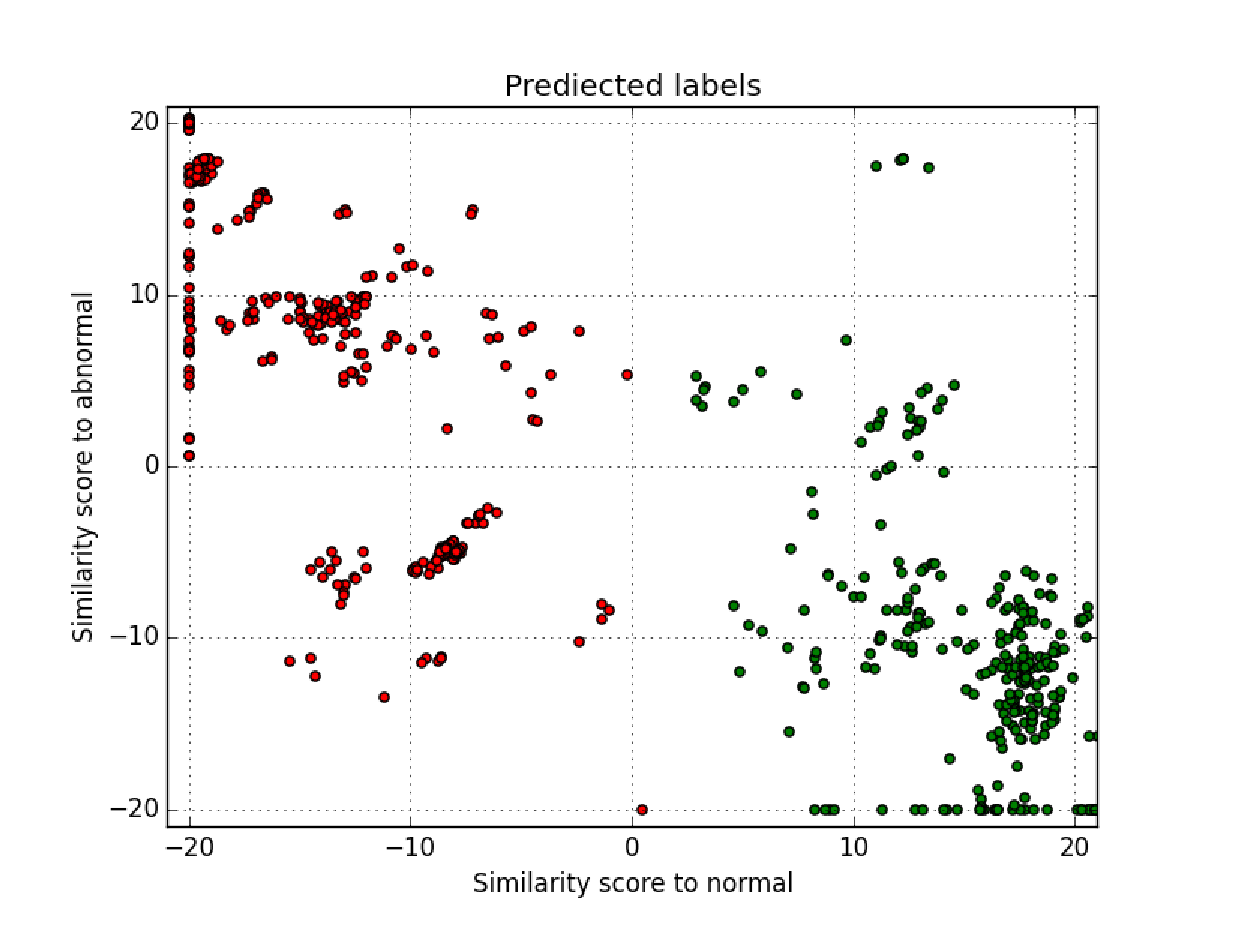
\includegraphics[width=3.0in,angle=0]{./sections/training20_test20_back_prediction_.eps}}
\subfloat[True labels]{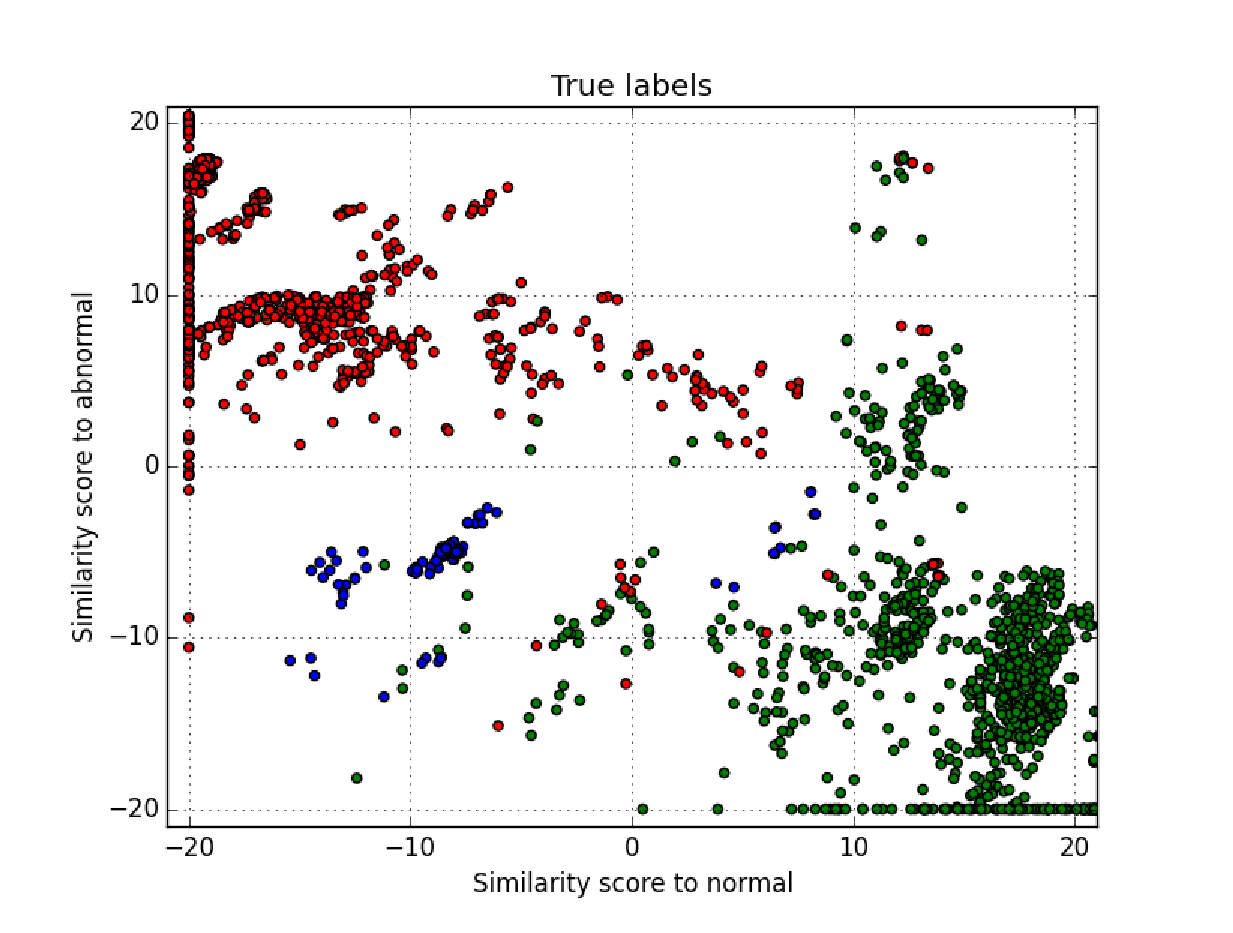
\includegraphics[width=3.0in,angle=0]{./sections/training20_test20_back_true_.eps}}
\end{center}
\caption{Anomaly detection for known anomalies. Red:Known and seen abnormal connections, Green:Known and seen normal connections, Blue:Intrusion "back" which is a known anomaly but in the testset.} % I may show rest of data in appendix
\label{fig:refSingleRobot1}

\end{figure}
\begin{table}[!ht]
\begin{center}
\begin{singlespace}
\scalebox{0.7}{
\begin{tabular}{| l | l | l | l | l | l | p{5cm} |}
\hline
Type of Anomaly & Number & TP & TN & FP & FN & Detection rate ($\%$ correct) \\
\hline
guess passwd & 1231 & 898 & 2158 (1231) & 35 (0) & 140 & 100 \\
\hline
ftp write & 3 & 1019 & 921 (1) & 44 (2) & 19 & 33.3 \\
\hline
nmap & 73 & 1002 & 997 (73) & 38 (0) & 36 & 100 \\
\hline
back & 370 & 1011 & 1280 (358) & 41 (12) & 27 & 96.7 \\
\hline
multihop & 18 & 1011 & 937 (15) & 43 (3) & 27 & 83.3 \\
\hline
rootkit & 13 & 1019 & 920 (0) & 55 (13) & 19 & 0  \\
\hline
pod & 41 & 1013 & 963 (41) & 40 (0) & 25 & 100 \\
\hline
perl & 2 & 1021 & 907 (0) & 57 (2) & 17 & 0 \\
\hline
ipsweep & 207 & 999 & 1041 (184) & 62 (23) & 39 & 88.8 \\
\hline
teardrop & 12 & 1021 & 932 (12) & 42 (0) & 17 & 100 \\
\hline
satan & 779 & 1015 & 1657 (777) & 40 (2) & 23 & 99.7 \\
\hline
loadmodule & 2 & 1011 & 924 (2) & 40 (0) & 27 & 100  \\
\hline
buffer overflow & 20 & 1012 & 940 (16) & 42 (4) & 26 & 80 \\ 
\hline
phf & 2 & 1019 & 908 (1) & 56 (1) & 19 & 50  \\
\hline
warezmaster & 944 & 946 & 1834 (908) & 72 (36) & 92 & 96.1 \\ 
\hline
imap & 1 & 1019 & 907 (0) & 56 (1) & 19 & 0 \\
\hline
warezclient & 22 & 1019 & 907 (0) & 55 (22) & 19 & 0 \\
\hline
land & 7 & 1021 & 914 (7) & 55 (0) & 17 & 100  \\
\hline
neptune & 5331 & 933 & 5588 (5327) & 31 (4) & 105 & 99.9 \\
\hline
smurf & 665 & 1018 & 1579 (665) & 48 (0) & 20 & 100  \\
\hline
\end{tabular}
}
\end{singlespace}
\end{center}
\caption{Known anomalies detection rate}
\label{fig:refSingleRobot1}
\end{table}

%Result provides the sensitivity and the coverage of similarity measure that is effective. 
%All data point in testset for 21 known abnomal classes shows similar to known anomalies. 
%After it calcurate the similarity among data points 
%\begin{table}[h]
%\begin{center}
%\begin{tabular}{| l | l | l | p{5cm} |}
%\hline
%Type of Anomaly & Predicted normal & Predicted anormalies & $\%$ correct\\
%\hline
%True normal &  &  & \\
%\hline
%True anormalies &  &  & \\
%\hline
%\end{tabular}
%\end{center}
%\caption{Abnomal classes in NSL-KDD99}
%\label{fig:refSingleRobot1}
%\end{table}
% The detection rate for them are quite high. 
%
%\begin{figure}[htb2]
%\begin{center}
%\end{center}
%\caption{Clusters of connections including known anomalies. The x-axis shows the normal similarity scores and the y-axis shows the known abnormal similarity scores}
%\label{fig:refSingleRobot1}
%\end{figure}
\newpage
\subsubsection{Unknown Anomalies}
We see that normal and abnormal connection similarity are also sensitive to most of unknown anomaly. 
However, we have four classes that are similar to normal connections. 
Connection density similarity measure is sensitive in this type of anomaly if it is above its threshold. 

13 out of 17 unknown anomalies such as "processtable" class are similar to known anomalies. 
Therefore we can detect them with exactly same way what it have done to known anomalies. 
Those results are good as known anomalies. 

\begin{table}[h]
\begin{center}
\scalebox{0.7}{
\begin{tabular}{| l | l | l | l | l | l | p{5cm} |}
\hline
Type of Anomaly & Number & TP & TN & FP & FN & Detection rate ($\%$ correct) \\
\hline
processtable & 685 & 1018 & 1597 (683) & 50 (2) & 20 & 99.7 \\ 
\hline
named & 17 & 1021 & 924 (4) & 55 (13) & 17 & 23.5\\
\hline
udpstorm & 2 & 1011 & 924 (2) & 40 (0) & 27 & 100 \\
\hline
sqlattack & 2 & 1021 & 907 (0) & 57 (2) & 17 & 0  \\
\hline
ps & 15 & 1019 & 910 (3) & 67 (12) & 19 & 20 \\
\hline
httptunnel & 133 & 1015 & 1016 (109) & 79 (24) & 23 & 81.9  \\
\hline
apache2 & 737 & 1014 & 1656 (734) & 43 (3) & 24 & 99.5 \\
\hline
saint & 319 & 1014 & 1227 (309) & 54 (10) & 24 & 96.8 \\
\hline
mscan & 996 & 1018 & 1910 (996) & 48 (0) & 20 & 100 \\
\hline
xterm & 13 & 1011 & 935 (13) & 40 (0) & 27 & 100  \\
\hline
worm & 2 & 1019 & 907 (0) & 57 (2) & 19 & 0 \\
\hline
xlock & 9 & 1013 & 925 (3) & 46 (6) & 25 & 66.66  \\
\hline
xsnoop & 4 & 1013 & 925 (3) & 41 (1) & 25 & 75  \\
\hline
\end{tabular}
}
\end{center}
\caption{Unknown anomalies that is similar to the known anomalies detection rate}
\label{fig:refSingleRobot1}
\end{table}

However 4 out of 17 are close to the normal connections in the training set. 
In that case, a cluster resulted by spectral clustering is denser than normal case can be detected by density based algorithm if we compare with mixture density generated by normal connections only. 
So with those prior knowledge we can use a spectral approach to find abnormal clusters which is originally classified as normal clusters. 

\begin{figure}[htb2]
\begin{center}
\subfloat[Predicted labels]{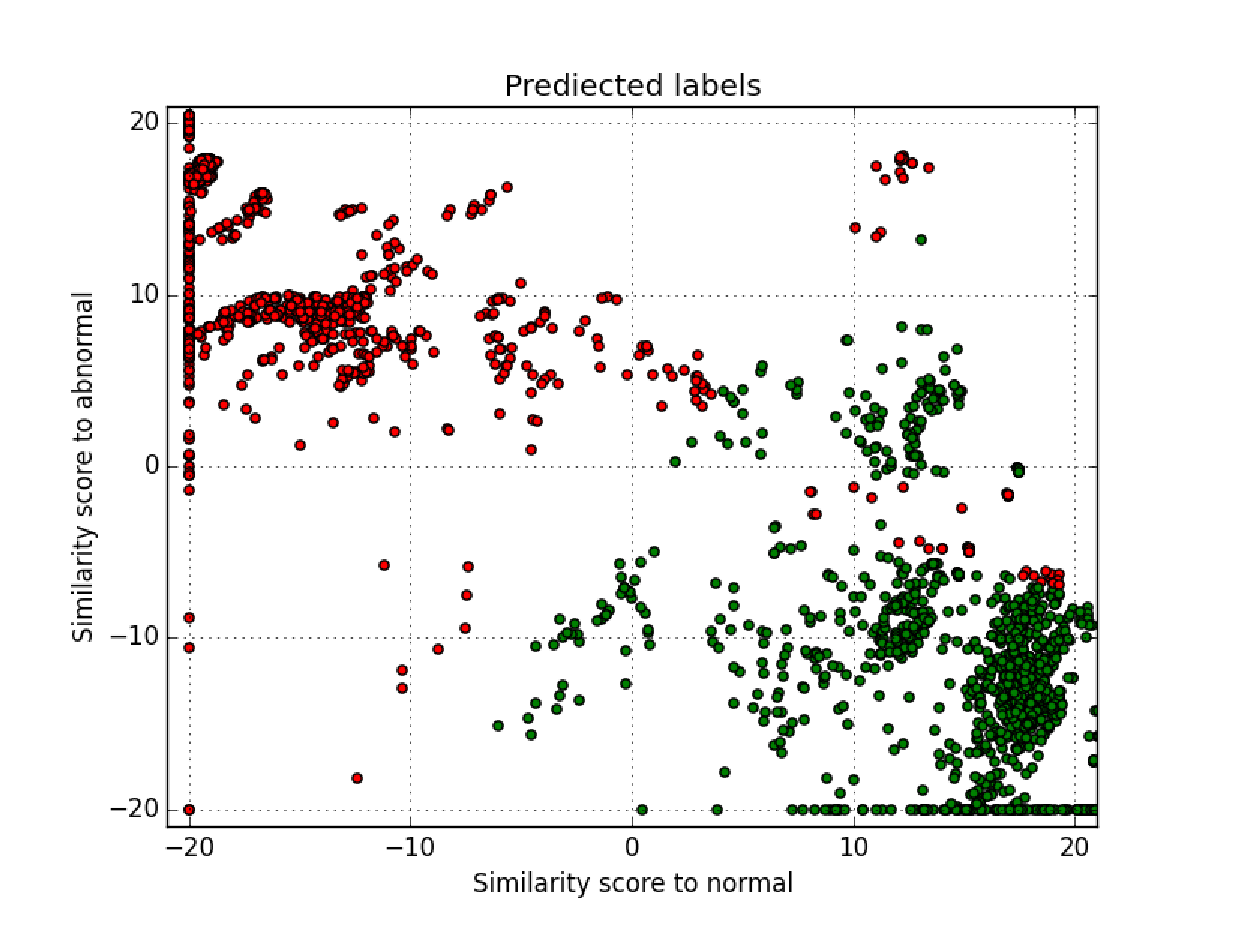
\includegraphics[width=2.0in,angle=0]{./sections/training20_test20_snmpguess_prediction_.eps}}
\subfloat[True labels]{\includegraphics[width=2.0in,angle=0]{./sections/training20_test20_snmpguess_true_.eps}}
\subfloat[Densities]{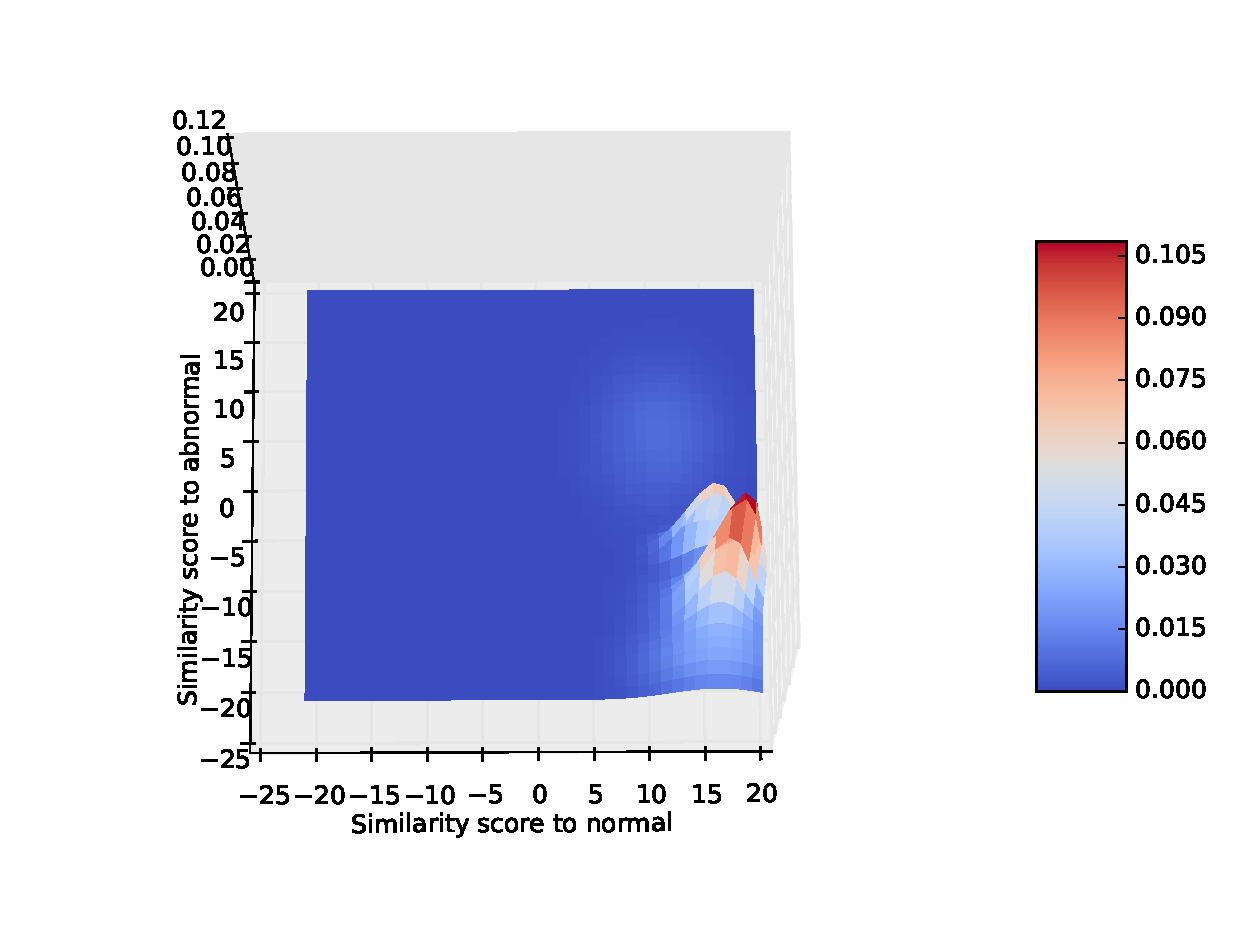
\includegraphics[width=2.0in,angle=0]{./sections/guess.eps}}
\end{center}
\caption{Density based intrusion detection result for unknown anomalies.  Red:Known and seen abnormal connections, Green:Known and seen normal connections, Blue:Intrusion "snmpguess" which is a unknown anomaly similar to normal connections.} % I may show rest of data in appendix
\label{fig:refSingleRobot1}
\end{figure}

The performance of density approach is not as good as previous one, and we can see that it is not able to detect "sendmail" class which is too few to form enough density. 
\begin{table}[h]
\begin{center}
\scalebox{0.7}{
\begin{tabular}{| l | l | l | l | l | l | p{5cm} |}
\hline
Type of Anomaly & Number & TP & TN & FP & FN & Detection rate ($\%$ correct) \\
\hline
snmpguess & 331 & 975 & 1182 (254) & 111 (77) & 63 & 76.7 \\ 
\hline
snmpgetattack & 178 & 973 & 1048 (126) & 92 (52) & 65 & 71.5 \\
\hline
mailbomb & 293 & 882 & 1133 (223) & 122 (70) & 156 & 76.1 \\
\hline
sendmail & 14 & 1019 & 907 (0) & 69 (14) & 19 & 0  \\
\hline
\end{tabular}
}
\end{center}
\caption{Unknown anomalies that is similar to known normals detection rate}
\label{fig:refSingleRobot1}
\end{table}

%4 out of 17 are close to known normal connections. 
%We can not detect them with exactly same way what it have done to known anomalies since abnormal and normal connections are mixed together. 
%However we can differenciate with density approach after the spectral clustering. 
%Here is the result, and their performance is good. 
%\begin{table}[h]
%\begin{center}
%\begin{tabular}{| l | l | l | p{5cm} |}
%\hline
%Type of Anomaly & Predicted normal & Predicted anormalies & $\%$ correct\\
%\hline
%True normal &  &  & \\
%\hline
%True anormalies (close to A)&  &  & \\
%\hline
%True anormalies (close to N) &  &  & \\
%\hline
%\end{tabular}
%\end{center}
%\caption{Abnomal classes in NSL-KDD99}
%\label{fig:refSingleRobot1}
%\end{table}
%\begin{table}[h]
%\begin{center}
%\begin{tabular}{| l | l | p{5cm} |}
%\hline
%Type of Anomaly & Count & $ \%$ correct\\
%\hline
%guess passwd & 100 & 80 \\
%\hline
%ftp write & 3 & 66.66 \\
%\hline
%nmap & 73 & 85.71 \\
%\hline
%back & 100 & 98.03  \\
%\hline
%multihop & 18 & 100  \\
%\hline
%rootkit & 13 & 84.61  \\
%\hline
%pod & 41 & 100  \\
%\hline
%perl & 2 & 0  \\
%\hline
%ipsweep & 117 & 97.4  \\
%\hline
%teardrop & 12 & 100  \\
%\hline
%satan & 100 & 87.96  \\
%\hline
%loadmodule & 2 & 0  \\
%\hline
%buffer overflow & 20 & 90  \\
%\hline
%phf & 2 & 50  \\
%\hline
%warezmaster & 100 & 84  \\
%\hline
%imap & 1 & 100  \\
%\hline
%warezclient & 6 & 0  \\
%\hline
%land & 7 & 100  \\
%\hline
%neptune & 100 & 100  \\
%\hline
%smurf & 100 & 100  \\
%\hline
%processtable & 100 & 100  \\
%\hline
%named & 17 & 88  \\
%\hline
%udpstorm & 2 & 100  \\
%\hline
%snmpguess & 100 & 72  \\
%\hline
%sqlattack & 2 & 100  \\
%\hline
%ps & 15 & 100  \\
%\hline
%httptunnel & 100 & 81  \\
%\hline
%sendmail & 14 & 0  \\
%\hline
%snmpgetattack & 100 & 97  \\
%\hline
%apache2 & 100 & 100  \\
%\hline
%saint & 100 & 98  \\
%\hline
%mailbomb & 100 & 72  \\
%\hline
%mscan & 100 & 100  \\
%\hline
%xterm & 13 & 100  \\
%\hline
%worm & 2 & 0  \\
%\hline
%xclock & 9 & 88.88  \\
%\hline
%xsnoop & 4 & 0  \\
%\end{tabular}
%\end{center}
%\caption{Abnomal classes in NSL-KDD99}
%\label{fig:refSingleRobot1}
%\end{table}

%\section{Conclusion}
%Summarize the entire report. 
%(Summarize the entire report)
Spectral approach for intrusion detection is presented. 
The unsupervised definition of anomalies used in the report is 
\begin{inparaenum}[\itshape a\upshape)]
\item the pattern dissimiliar to the majority of normal patterns, 
\item and infrequently occurred density.
\end{inparaenum}
Graph Laplacian captures those patterns well from the data tranported by EM algorithm. 
Experimental results on NSL-KDD data set indicate that similarity measurement approach is very effective both unseen known type of anomalies and unseen unknown type of anomalies. 
The number of cluster does not always best from its eigengap when the data have considerable noises. 
So one-to-one clustering is not applicable because of the limitation of eigensolver's sensitivity. 
%limitations of eigensolver's sensitivity, one-to-one clustering is not applicable when the data have considerable noises.
The proposed algorithm with multiclass spectral clustering has better detection performance than that of one-to-one spectral clustering. 
%However, multiclass spectral clustering's performance is good on those situation. %the number of cluster is fixed. 
%The approximated k-NN might improve the applicability.
%The proposed algorithm has the same detection performace as (sth), but it is (sth) efficient.

% (Future work)
%% Outline what needs to/can be done in the future.
Future work on more robust multi-class approach is needed. 
More specifically, it would be interesting to design an algorithm with robust eigensolver, where the most noise will have the highest influence on the clustering performance. 
In addtion, an extension of density sensitive similarity function is also worth considering. 
%(salability, sensitivity, coverage)

%-----------------------
\newpage
\begin{thebibliography}{9}

% Introduction. Report from verizon. Why this subject is important.
\bibitem{verizon14}
\emph{"2014 Data Breach Investigations Report"} Verizon (2014) %http://www.verizonenterprise.com/DBIR/2014/

% Related works. 
\bibitem{chandola09}
Chandola, Varun, Arindam Banerjee, and Vipin Kumar. \emph{"Anomaly detection: A survey."} ACM Computing Surveys (CSUR) 41.3 (2009): 15.

\bibitem{aggarwal01}
Aggarwal, Charu C., and Philip S. Yu. "Outlier detection for high dimensional data." ACM Sigmod Record. Vol. 30. No. 2. ACM, 2001.

\bibitem{ramaswamy00}
Ramaswamy, Sridhar, Rajeev Rastogi, and Kyuseok Shim. "Efficient algorithms for mining outliers from large data sets." ACM SIGMOD Record. Vol. 29. No. 2. ACM, 2000.

\bibitem{breuning00}
Breunig, Markus M., et al. "LOF: identifying density-based local outliers." ACM Sigmod Record. Vol. 29. No. 2. ACM, 2000.

% Dataset. 
\bibitem{tavallaee09}
Tavallaee, Mahbod, et al. \emph{"A detailed analysis of the KDD CUP 99 data set."} Proceedings of the Second IEEE Symposium on Computational Intelligence for Security and Defence Applications 2009. 2009
\bibitem{olusola10}
Olusola, Adetunmbi A., Adeola S. Oladele, and Daramola O. Abosede. "Analysis of KDD’99 Intrusion detection dataset for selection of relevance features." Proceedings of the World Congress on Engineering and Computer Science. Vol. 1. 2010.
\bibitem{kayacik05}
Kayacik, H. Günes, A. Nur Zincir-Heywood, and Malcolm I. Heywood. "Selecting features for intrusion detection: A feature relevance analysis on KDD 99 intrusion detection datasets." Proceedings of the third annual conference on privacy, security and trust. 2005.

% methods. Spectral clustering
\bibitem{jianbo00}
Jianbo Shi and Jitendra Malik, Normalized Cuts and Image Segmen- tation IEEE Transactions on Pattern Analysis and Machine Intelligence, 22(8)(2000) 888-905.

\bibitem{ng01}
Ng, Andrew Y., Michael I. Jordan, and Yair Weiss. "On spectral clustering: Analysis and an algorithm." Advances in neural information processing systems 2 (2002): 849-856.

\bibitem{jordan04}
Jordan, Francis R. Bach Michael I., and F. R. Bach. "Learning spectral clustering." Advances in Neural Information Processing Systems 16 (2004): 305-312.

\bibitem{dhillon04}
Dhillon, Inderjit S. and Guan, Yuqiang and Kulis, Brian, Kernel K-means, Spectral Clustering and Normalized Cuts, In Proceedings of the tenth ACM SIGKDD International conference on Knowledge discovery and data mining (KDD’04),(2004) 551-556.

\bibitem{cding04}
C.Ding and X. He. Linearized Cluster Assignment via Spectral Ordering, In proceedings of International Conference on Machine Learning, New York 2004.

\bibitem{ulrike07}
Von Luxburg, Ulrike. "A tutorial on spectral clustering." Statistics and computing 17.4 (2007): 395-416.

% methods. Outlier detection.
\bibitem{knorr00}
Knorr, Edwin M., Raymond T. Ng, and Vladimir Tucakov. "Distance-based outliers: algorithms and applications." The VLDB Journal—The International Journal on Very Large Data Bases 8.3-4 (2000): 237-253.

\end{thebibliography}

%-----------------------
\clearpage
%-----------------------
\end{document}
%-----------------------
